%%%%%%%%%%%%%%%%%%%%%%%%%%%%%%%%%%%%%%%%%%%%%%%%%%%%%%%%%%%%%%%%%%%%%%%%%%%%%%%%%%%%%%%%%%%%%%
% READ ME
% 
% 1. Please give details of your working group, institute, time schedule in the SPECIFICATION, see section A.
% 2.1 Load the content package of your language in section E.
% 2.2 Load the individual files one after the other and compile.  
% 2.3 Comile the lecture matieral with LuaLaTeX and the worksheet material with pdfLaTeX (!)
%%%%%%%%%%%%%%%%%%%%%%%%%%%%%%%%%%%%%%%%%%%%%%%%%%%%%%%%%%%%%%%%%%%%%%%%%%%%%%%%%%%%%%%%%%%%%%

\documentclass[xcolor=dvipsnames]{beamer}

%%%%%%%%%%%%%%%%%%%%%%%%%%%%%%%%%%%%%%%%%%%%%%%%%%%%%%%%%%%%%%%%%%%%%%%%%%%%%%%%%%%%%%%%%%%%%%
% [A] PLEASE FILL IN THE GAPS IN THE SPECIFICATION.TEX
%%%%%%%%%%%%%%%%%%%%%%%%%%%%%%%%%%%%%%%%%%%%%%%%%%%%%%%%%%%%%%%%%%%%%%%%%%%%%%%%%%%%%%%%%%%%%%


%%%%%%%%%%%%%%%%%%%%%%%%%%%%%%%%%%%%%%%%%%%%%%%%%%%%%%%%%%%%%%%%%%%%%%%%%%%%%%%%%%%%%%%%%%%%%%
% [A] PLEASE FILL IN THE GAPS
%%%%%%%%%%%%%%%%%%%%%%%%%%%%%%%%%%%%%%%%%%%%%%%%%%%%%%%%%%%%%%%%%%%%%%%%%%%%%%%%%%%%%%%%%%%%%%
% You can add two Logos, f.e. your university, insitute, working group, organisation (...) except the LHCb-Logo, it's still included and placed.

\newcommand*{\WorkGroup}{Ellinor Eckstein, Lukas Julian Exner, Ludwig Kramer, Niklas Kramer, \underline {Sebastian Neubert}, Piet Nogga} %f.i.: LHCb Bonn
\newcommand*{\WorkGroupWebsite}{https://www.hiskp.uni-bonn.de/?id=663} %f.i.: https://www.hiskp.uni-bonn.de/?id=663
\newcommand*{\University}{University of Bonn} %f.i.: University of Bonn
\newcommand*{\LogoUniversity}{
\includegraphics[height=1cm]{Logos And Group/University of Bonn_logo.png}}
\newcommand*{\LogoInsitute}{
\includegraphics[height=1cm]{Logos And Group/HISKP_Logo.jpg}}
\newcommand*{\dateMC}{07.03.2024} \date{\dateMC}
\newcommand*{\Event}{LHCb International Masterclass} %f.i.: International Masterclass


%If you have an overview of all your members, please insert a PDF (!) file here. If not: Leave it commented out. 
\newcommand*{\GroupPresentation}{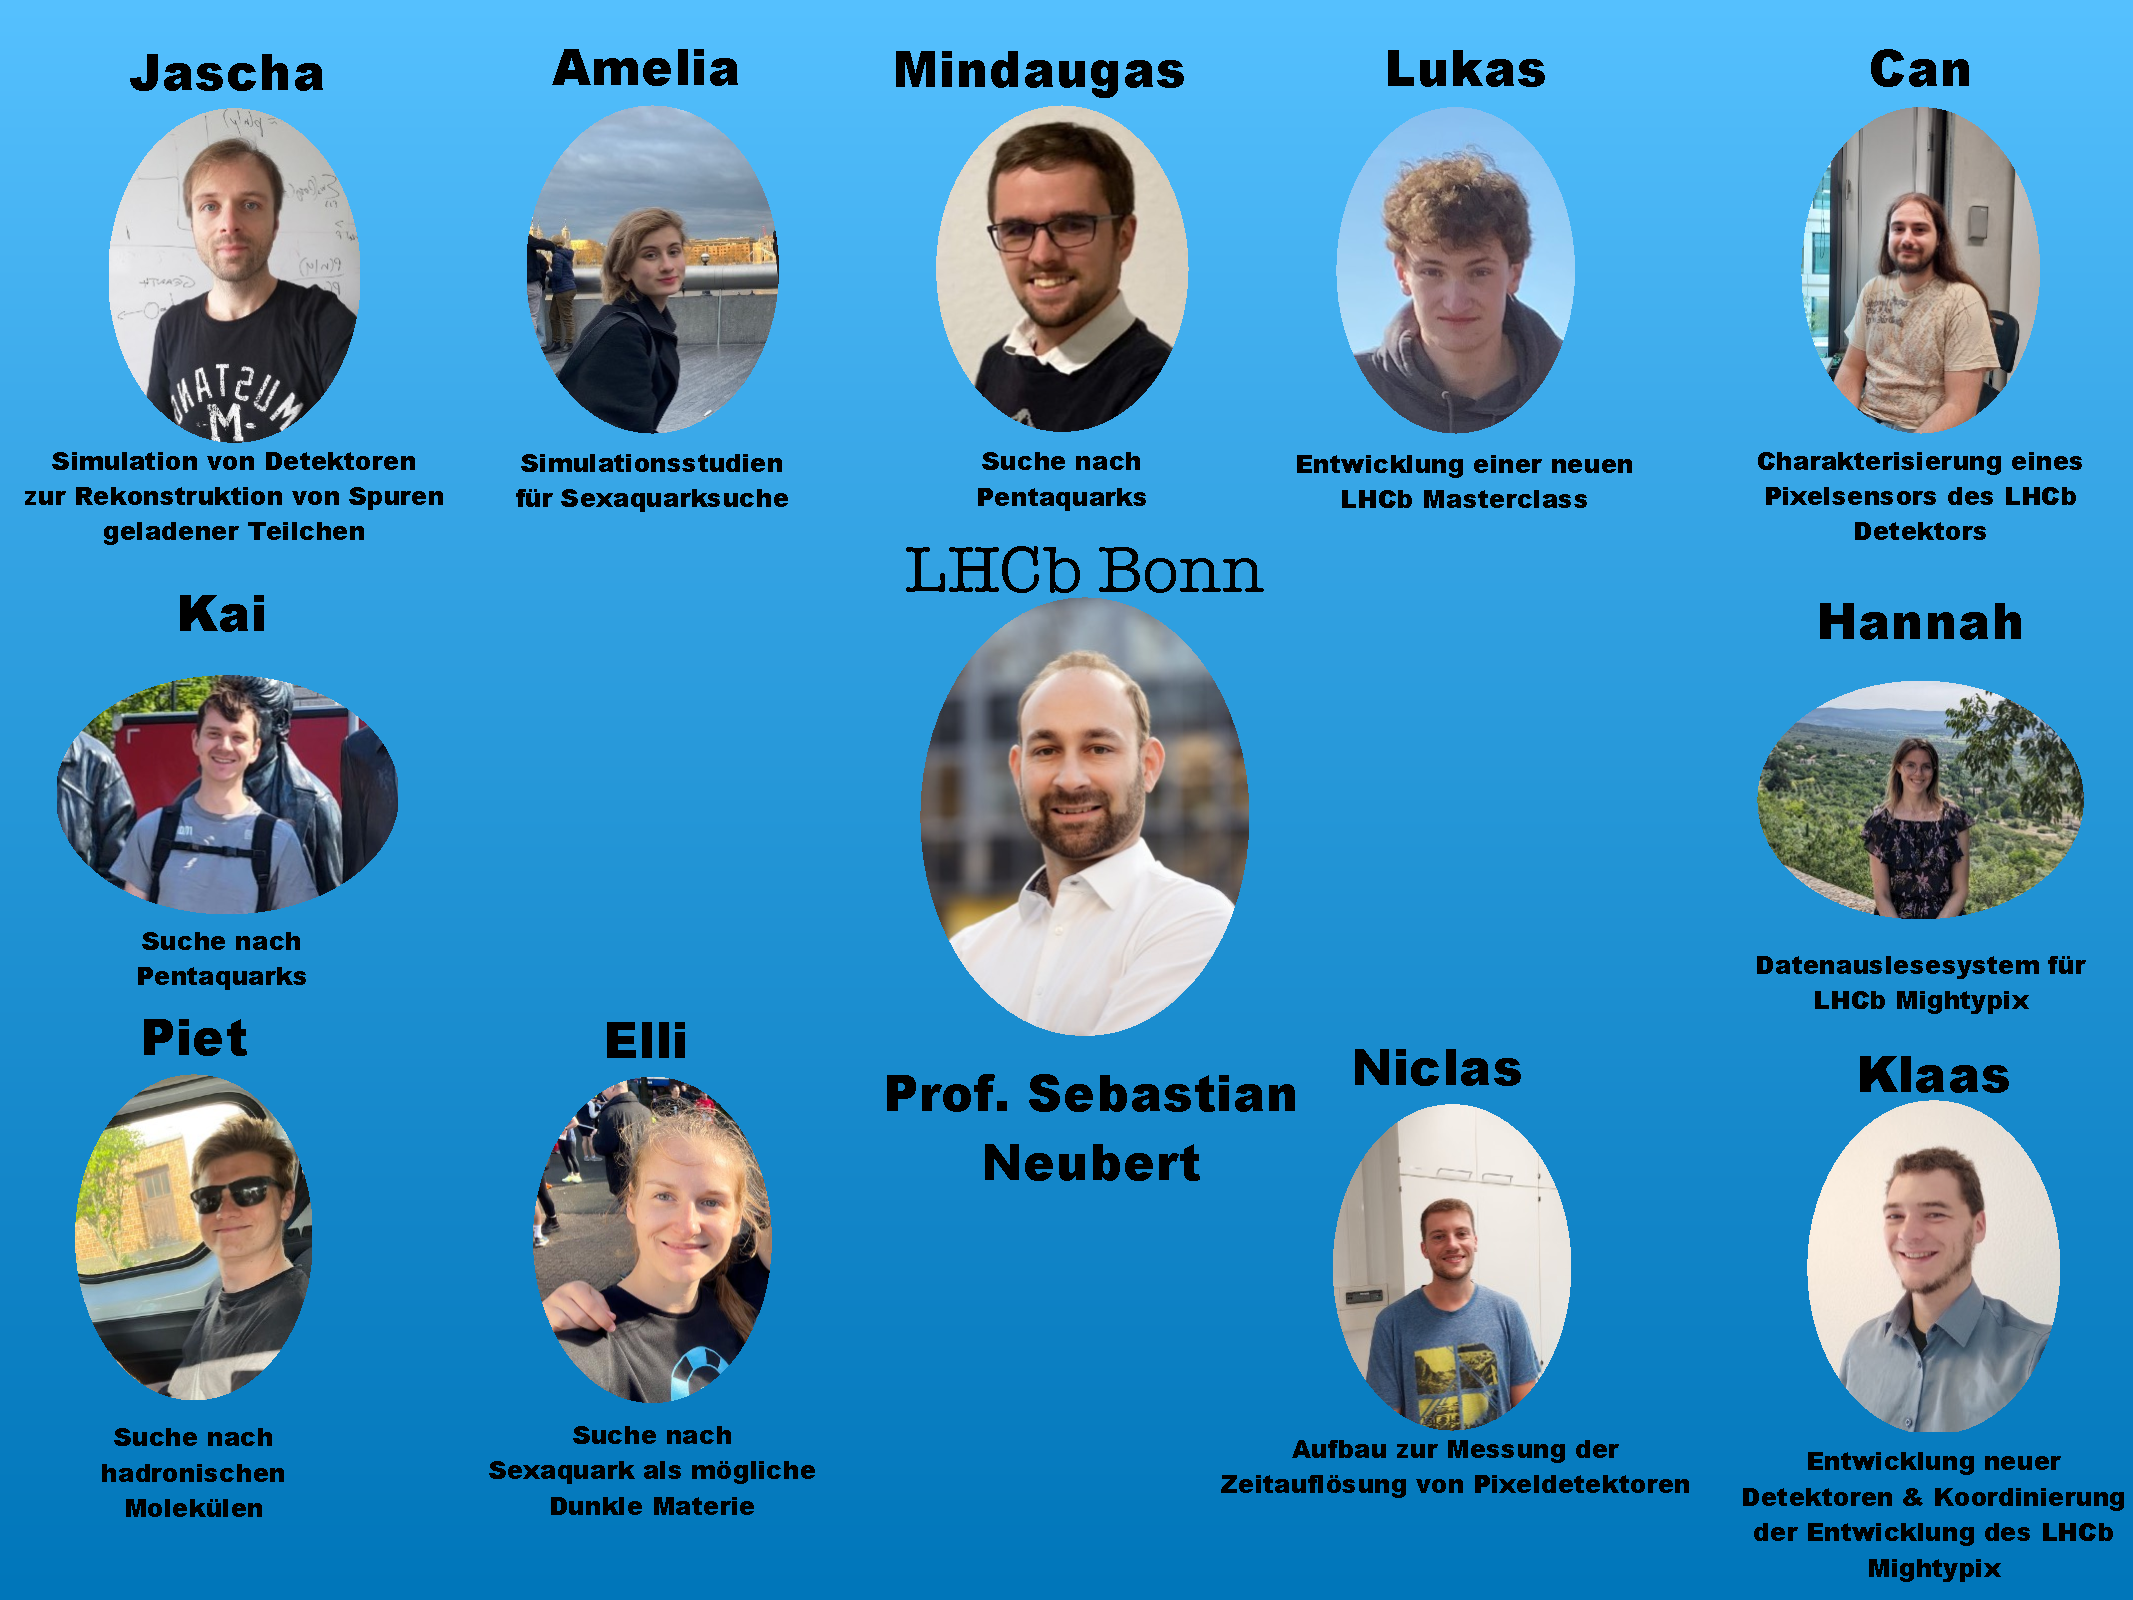
\includepdf[]{Logos And Group/Group_Pres.pdf}}

% Fill in the timetable

\newcommand*{\PersonIntroductory}{<Person1>}
\newcommand*{\PersonHadrons}{Ellinor Eckstein, \underline {Lukas Julian Exner}, Ludwig Kramer, Niklas Kramer, Sebastian Neubert, Piet Nogga}
\newcommand*{\PersonDataAnalysis}{\underline {Ellinor Eckstein}, \underline {Lukas Julian Exner}, Ludwig Kramer, Niklas Kramer, Sebastian Neubert, Piet Nogga}
\newcommand*{\PersonDiscusion}{Ellinor Eckstein, Lukas Julian Exner, Ludwig Kramer, Niklas Kramer, Sebastian Neubert, Piet Nogga}





%%%%%%%%%%%%%%%%%%%%%%%%%%%%%%%%%%%%%%%%%%%%%%%%%%%%%%%%%%%%%%%%%%%%%%%%%%%%%%%%%%%%%%%%%%%%%%


%%%%%%%%%%%%%%%%%%%%%%%%%%%%%%%%%%%%%%%%%%%%%%%%%%%%%%%%%%%%%%%%%%%%%%%%%%%%%%%%%%%%%%%%%%%%%%
% [B]  DESIGN OF THE SLIDES
%%%%%%%%%%%%%%%%%%%%%%%%%%%%%%%%%%%%%%%%%%%%%%%%%%%%%%%%%%%%%%%%%%%%%%%%%%%%%%%%%%%%%%%%%%%%%%
%Colours
\definecolor{VELO}{RGB}{205,200,0}
\definecolor{RICH}{RGB}{244,177,131}
\definecolor{Magnet}{RGB}{0,112,192}
\definecolor{ECAL}{RGB}{0,176,240}
\definecolor{HCAL}{RGB}{0,112,192}
\definecolor{Muon}{RGB}{0,176,80}
\definecolor{Proton}{RGB}{0,58,232}
\definecolor{upQuark}{RGB}{11,140,91}
\definecolor{downQuark}{RGB}{0,0,0}
\definecolor{strangeQuark}{RGB}{153,1,153}
\definecolor{Elektron}{RGB}{246,123,40}

\definecolor{LHCbRed}{RGB}{220,40,37}
\definecolor{LHCbLightBlue}{RGB}{214,242,252}
\definecolor{LHCbDarkBlue}{RGB}{33,84,172}

%Design
\usetheme{Madrid}
%\useoutertheme{miniframes} % Alternatively: miniframes, infolines, split
%\useinnertheme{circles}
\usepackage{tcolorbox}
\newcommand{\n}[1]{\textmd{#1}}
\definecolor{darkblue}{rgb}{0.04706, 0.13725, 0.26667} 
\definecolor{darkgreen}{rgb}{0,0.65,0.4}
\definecolor{lightgreen}{rgb}{0.85, 0.86, 0.1}
\definecolor{lightgray}{rgb}{0.9, 0.9, 0.9} 
\setbeamercolor{palette primary}{bg=lightgray,fg=black}
\setbeamercolor{palette secondary}{bg=white,fg=white}
\setbeamercolor{palette tertiary}{bg=white,fg=white}
\setbeamercolor{palette quaternary}{bg=yellow,fg=white}
\setbeamertemplate{navigation symbols}{}
\setbeamercolor{structure}{bg=lightgray,fg=black}
\setbeamercolor{section in toc}{fg=Black}
\setbeamercolor{subsection in head/foot}{bg=Black,fg=gray}
\setbeamercolor{background canvas}{bg=white}
\setbeamercolor{normal text}{fg=darkblue}
\usebeamercolor*{normal text}
\setbeamertemplate{itemize subsubitem}{\tiny\ding{109}}
\setbeamertemplate{itemize item}{\tiny\ding{108}}%\setbeamertemplate{itemize items}[ball]







\newcommand{\textbg}[1]{\par\noindent\colorbox{lightgray}
{\parbox{\dimexpr\textwidth-2\fboxsep\relax}{#1}}}
%%%%%%%%%%%%%%%%%%%%%%%%%%%%%%%%%%%%%%%%%%%%%%%%%%%%%%%%%%%%%%%%%%%%%%%%%%%%%%%%%%%%%%%%%%%%
% [C] BASIC PACKAGES
%%%%%%%%%%%%%%%%%%%%%%%%%%%%%%%%%%%%%%%%%%%%%%%%%%%%%%%%%%%%%%%%%%%%%%%%%%%%%%%%%%%%%%%%%%%%
\usepackage[english, ngerman]{babel}
\usepackage{caption}
\usepackage{multicol}
\usepackage{ragged2e}
\usepackage[export]{adjustbox}
\usepackage{multimedia}
\usepackage{media9}
\usepackage{hyperref}
\usepackage{pifont}
\usepackage{tikz} 
\usepackage{overpic}
\usepackage{pgfplots}
\usepackage{pdfpages}
\usepackage{siunitx}
\pgfplotsset{width=15cm,compat=1.9}
\usepackage{tikz-feynman}
\usepackage[nottoc]{tocbibind}
\usepackage{nicefrac}
\usepackage{setspace}
\usepackage{movie15}
\usepackage{animate}
\usepackage{graphicx, animate}
\usepackage{multimedia}
\usepackage[table]{xcolor}
\usefonttheme{professionalfonts}
\usepackage{soul}
\usepackage{pgfplotstable}
\tikzset{>=latex}
\usetikzlibrary{decorations.markings, calc}
%%%%%%%%%%%%%%%%%%%%%%%%%%%%%%%%%%%%%%%%%%%%%%%%%%%%%%%%%%%%%%%%%%%%%%%%%%%%%%%%%%%%%%%%%%%%
% [D] FONT
%%%%%%%%%%%%%%%%%%%%%%%%%%%%%%%%%%%%%%%%%%%%%%%%%%%%%%%%%%%%%%%%%%%%%%%%%%%%%%%%%%%%%%%%%%%%
\usepackage[default]{comfortaa}
\usepackage[T1]{fontenc}
%\setsansfont{comfortaa}

\DeclareMathAlphabet{\mathrm}{OT1}{cmss}{m}{rm}

%%%%%%%%%%%%%%%%%%%%%%%%%%%%%%%%%%%%%%%%%%%%%%%%%%%%%%%%%%%%%%%%%%%%%%%%%%%%%%%%%%%%%%%%%%%%
% [E] IMPORT CONTENT
%%%%%%%%%%%%%%%%%%%%%%%%%%%%%%%%%%%%%%%%%%%%%%%%%%%%%%%%%%%%%%%%%%%%%%%%%%%%%%%%%%%%%%%%%%%%

\input{eng_Lecture_Introduction}



